%!TEX program = xelatex

\documentclass[a4paper, openany, oneside]{memoir}
\usepackage[no-math]{fontspec}
\usepackage{pgfplots}
\pgfplotsset{compat=newest}
\usepackage{commath}
\usepackage{mathtools}
\usepackage{amssymb}
\usepackage{amsthm}
\usepackage{booktabs}
\usepackage{mathtools}
\usepackage{xcolor}
\usepackage[separate-uncertainty=true, per-mode=symbol]{siunitx}
\usepackage[noabbrev, capitalize]{cleveref}
\usepackage{listings}
\usepackage[american inductor, european resistor]{circuitikz}
\usepackage{amsmath}
\usepackage{amsfonts}
\usepackage{ifxetex}
\usepackage[dutch,english]{babel}
\usepackage[backend=bibtexu,texencoding=utf8,bibencoding=utf8,style=ieee,sortlocale=en_GB,language=auto]{biblatex}
\usepackage[strict,autostyle]{csquotes}
\usepackage{parskip}
\usepackage{import}
\usepackage{standalone}
\usepackage{hyperref}
%\usepackage[toc,title,titletoc]{appendix}

\ifxetex{} % Fonts laden in het geval dat je met Xetex compiled
    \usepackage{fontspec}
    \defaultfontfeatures{Ligatures=TeX} % To support LaTeX quoting style
    \setromanfont{Palatino Linotype} % Tover ergens in Font mapje in root.
    \setmonofont{Source Code Pro}
\else % Terug val in standaard pdflatex tool chain. Geen ondersteuning voor OTT fonts
    \usepackage[T1]{fontenc}
    \usepackage[utf8]{inputenc}
\fi
\newcommand{\references}[1]{\begin{flushright}{#1}\end{flushright}}
\renewcommand{\vec}[1]{\boldsymbol{\mathbf{#1}}}
\newcommand{\uvec}[1]{\boldsymbol{\hat{\vec{#1}}}}
\newcommand{\mat}[1]{\boldsymbol{\mathbf{#1}}}
\newcommand{\fasor}[1]{\boldsymbol{\tilde{\vec{#1}}}}
\newcommand{\cmplx}[0]{\mathrm{j}}
\renewcommand{\Re}[0]{\operatorname{Re}}
\newcommand{\Cov}{\operatorname{Cov}}
\newcommand{\Var}{\operatorname{Var}}
\newcommand{\proj}{\operatorname{proj}}
\newcommand{\Perp}{\operatorname{perp}}
\newcommand{\col}{\operatorname{col}}
\newcommand{\rect}{\operatorname{rect}}
\newcommand{\sinc}{\operatorname{sinc}}
\newcommand{\IT}{\operatorname{IT}}
\newcommand{\F}{\mathcal{F}}

\newtheorem{definition}{Definition}
\newtheorem{theorem}{Theorem}


\DeclareSIUnit{\voltampere}{VA} %apparent power
\DeclareSIUnit{\pii}{\ensuremath{\pi}}

\hypersetup{%setup hyperlinks
    colorlinks,
    citecolor=black,
    filecolor=black,
    linkcolor=black,
    urlcolor=black
}

% Example boxes
\usepackage{fancybox}
\usepackage{framed}
\usepackage{adjustbox}
\newenvironment{simpages}%
{\AtBeginEnvironment{itemize}{\parskip=0pt\parsep=0pt\partopsep=0pt}
\def\FrameCommand{\fboxsep=.5\FrameSep\shadowbox}\MakeFramed{\FrameRestore}}%
{\endMakeFramed}

% Impulse train
\DeclareFontFamily{U}{wncy}{}
\DeclareFontShape{U}{wncy}{m}{n}{<->wncyr10}{}
\DeclareSymbolFont{mcy}{U}{wncy}{m}{n}
\DeclareMathSymbol{\Sha}{\mathord}{mcy}{"58}
\addbibresource{../../../includes/bibliography.bib}

\title{Compressive Sensing - An Overview}

\author{W.P. Bruinsma \and R.P. Hes \and H.J.C. Kroep \and T.C. Leliveld \and W.M. Melching \and T.A. aan de Wiel}

\raggedbottom

\begin{document}
\chapter{Model - Cogradio}
\label{cha:model}
In this chapter we will discuss the model part of our system. All the software discussed in this chapter is contained in \lib{cogradio} in the source. We will describe each step of the process from sampling to detection. For each step we will describe which methods we used and what choices we made.

\section{Source}
\label{sec:source}
All our sources are derived from one base source, that defines the methods that every source should implement: the constructor and a \func{generate} function. This generate function should return the requested number of samples from a specific source. The rest of our source can be divided in two categories, the simulated sources used for testing our algorithms and real-world sources that connect to the USRPs to retrieve samples.

\begin{figure}
    \centering
    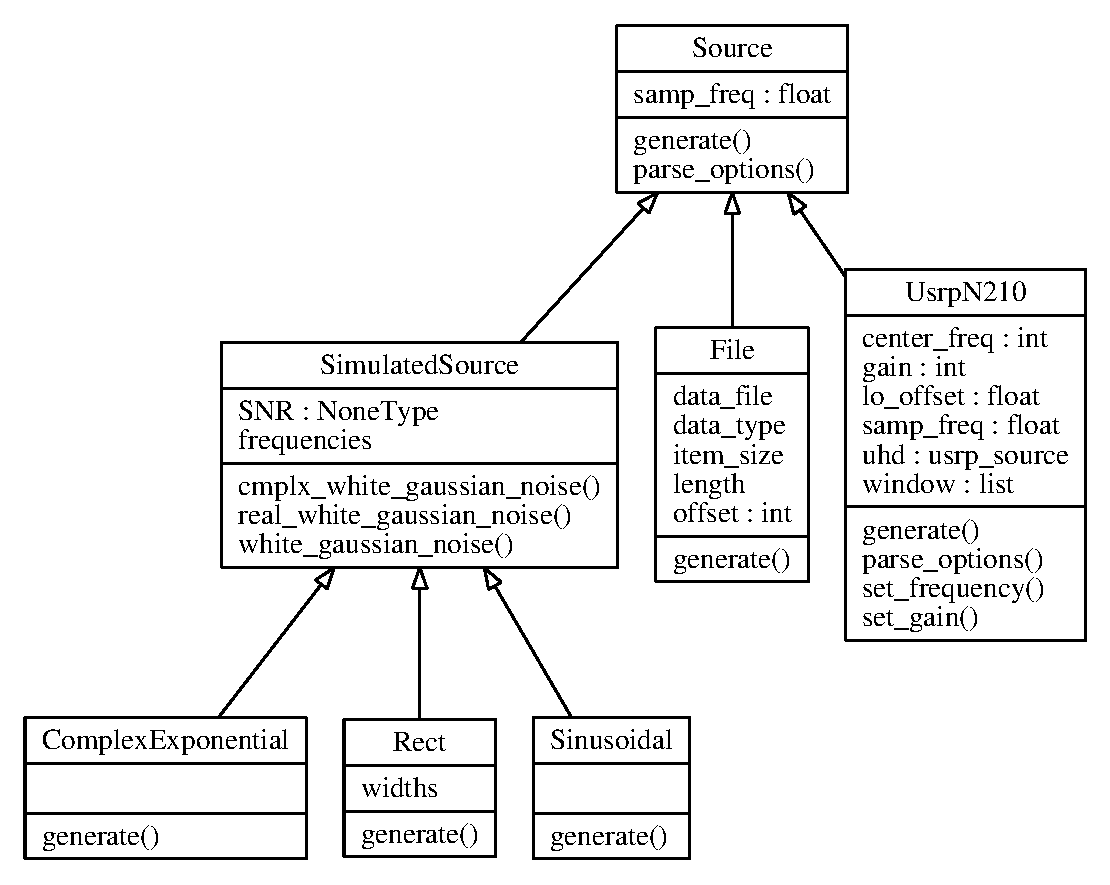
\includegraphics[width=\linewidth]{figures/classes_source.eps}
    \caption{The UML diagram of the sources.}
    \label{fig:umlsource}
\end{figure}

\subsection{Simulated Source}
\label{sec:simulated-source}
The simulated sources are used for testing our algorithms. They generate samples on the fly, or use pre-recorded data. All the simulated sources have the same base class: \func{SimulatedSource}. This base class adds some utility methods to the sources to add Gaussian noise to the generated data.

\subsubsection{Sinusoidal}
The sinusoidal source generates a real valued signal, with a sum of sinusoidal signals with different frequencies. Because the signal is real valued this generates a symmetrical spectrum.

\subsubsection{Complex exponential}
The complex exponential source is the complex equivalent of the sinusoidal source. The generated complex signal is the sum of complex exponentials with different frequencies,

\subsubsection{Rectangular source}
The rectangular source generates a signal with multiple rectangles in the spectrum with specified frequencies and widths. The time domain signal is generated by adding multiple sinc functions.

\subsubsection{File source}
The file source reads the samples from a file. This was used to test with real world data, but still get reproducible results. The files can be generated with \lib{GNU Radio} using a file sink.


\subsection{USRP source}
For the USRPs we have two sources. One for normal operation for simulating different sampling methods. The other is for doing hardware co-prime sampling. The USRP sources also have methods to change the centre frequency and the gain of the front-end of the radio.

\subsubsection{Normal source}
The normal source uses the \func{finite\_acquisition} function. This provides a very easy way to get a specified number of samples from one USRP\@. This method has a few drawbacks (see \cref{sec:drivers}). The problems with the dc compensation of the local oscillator are prevented by shifting the local oscillator out of the sampled spectrum. Unfortunately this halves our effective bandwidth.

\subsubsection{Coprime source}
The coprime source uses an external \CC~program to do the actual sampling. This program synchronises the two streams and can sample from two USRPs with different sample rates. The samples are then sent over a socket to the coprime source in Python for further processing.


\section{Sampling}
\label{sec:sampling}
After the samples are generated, different sampling methods have to be applied. In most cases this consists of reshaping the input vector and throwing samples out. To compare different methods we wrote samplers for simulated multi-coset, simulated coprime and coprime with data from two sources. Each sampler is inherited from a base class called \func{Sampler}. This base class defines the three used methods, the constructor, a \func{sample} method to act on the input samples, and a \func{get\_C} function to generate a sampling matrix for the reconstructor that corresponds to the sampling method.

\begin{figure}
    \centering
    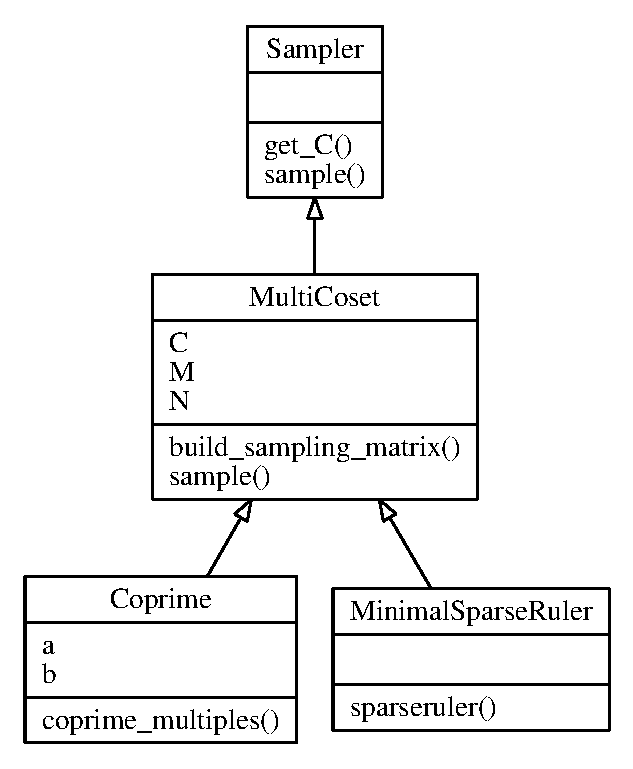
\includegraphics{./figures/classes_sampling.eps}
    \caption{The UML diagram of the samplers.}
    \label{fig:}
\end{figure}

\subsection{Multi-coset sampler}
\label{sec:multi-coset-sampler}
The multi-coset sampler first chooses a sparse ruler according to its input arguments. With this sparse ruler a sampling matrix is constructed, as in Section ***. The output is then generated by multiplying the input vector by this sampling matrix.

\subsection{coprime sampler}
\label{sec:coprime-sampler}
The coprime sampler works in the same way as the multi-coset sampler. The only difference is the way the sampling matrix is constructed. This is done as in Section ***.

\subsection{Hardware coprime}
\label{sec:hardware-coprime}
The hardware coprime sampler does not get one vector with input samples, but two with a different number of samples from two samplers with different sample rates. The sampling matrix is constructed as with the normal coprime sampler. The two input vectors are then transformed in one output vector that matches the sampling matrix.

\section{Reconstruction}
\label{sec:reconstruction}
Two different kind of reconstruction methods are implemented. One similar to the one specified in \cite{ariananda2012compressive} the other is discussed in Part 1 of this thesis. Both reconstructors implement the interface \func{reconstructor} which has a contract for one method named \func{reconstruct(signal)}. Both classes make use of the shared function \func{calc\_pseudoinverse(R)}. This is a wrapper around \lib{SciPy's} \func{pinv}, which calculates the pseudoinverse. Because this operation is quite time consuming for larger systems a caching mechanism was introduced to lower startup times.

\subsection{CrossCorrelation}
\label{sub:crosscorrelation}
The CrossCorrelation class implementation is based on \cite{ariananda2012compressive}. Its constructor generates its pseudoinverse similarly to how it is described in the paper. It's implementation of \func{reconstruct(signal)} is rather straightforward using a simple matrix multiplication to solve the system.

\subsection{Wessel}
\label{sub:wessel}
Wessel's reconstructor is a variation on the reconstruction technique implemented by \func{CrossCorrelation}. The theory is thoroughly described in the first part of this thesis. The constructor takes 3 arguments (one optional):
\begin{description}
    \item[L] determines the maximum lag estimated of cross-correlation of the cosets.
    \item[C] is the sampling matrix used by one of the samplers. This is required for the reconstruction algorithm.
    \item[cache] (default is True) is a boolean value that determines whether the pseudo-inverse can be loaded and saved to the cache. Mainly used for test and profiling purposes.
\end{description}
The constructor gets the number of cosets and the down-sampling factor from the C matrix. It constructs the R matrix in \func{constructR()}, which makes use of the \func{build\_D()}, \func{filter\_cross\_correlations()} and \func{build\_rcc()} as helper functions.

The \func{reconstruct(signal)} takes the pseudo-inverse and multiplies it with output of \func{cross\_correlation\_signals(signal)} reshaped to a vector. This is the functionality as described in \cref{cha:reconstruction}.

\begin{figure}
    \centering
    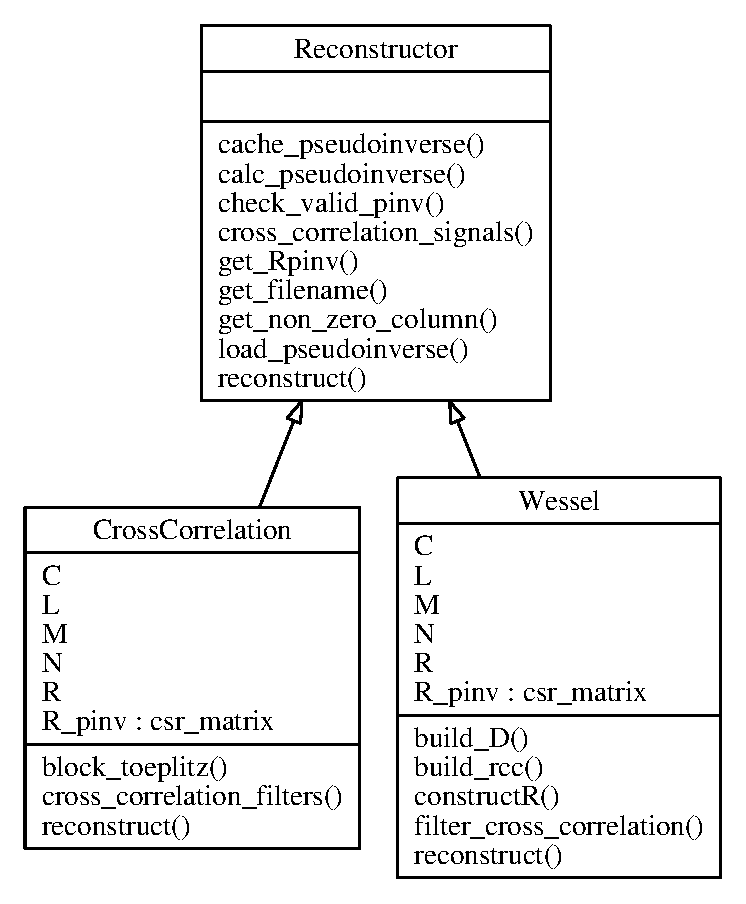
\includegraphics{./figures/classes_reconstruction.eps}
    \caption{The UML diagram of the reconstructors.}
    \label{fig:umlreconstructor}
\end{figure}

\section{Detection}
\label{sec:detection}

\begin{figure}
    \centering
    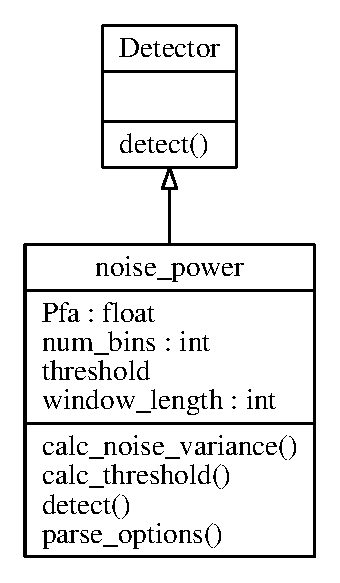
\includegraphics{./figures/classes_detection.eps}
    \caption{The UML diagram of the detectors.}
    \label{fig:umldetector}
\end{figure}

\section{Utilities}
\label{sec:utilities}


\end{document}
